% Created by tikzDevice version 0.7.0 on 2014-09-12 17:45:09
% !TEX encoding = UTF-8 Unicode
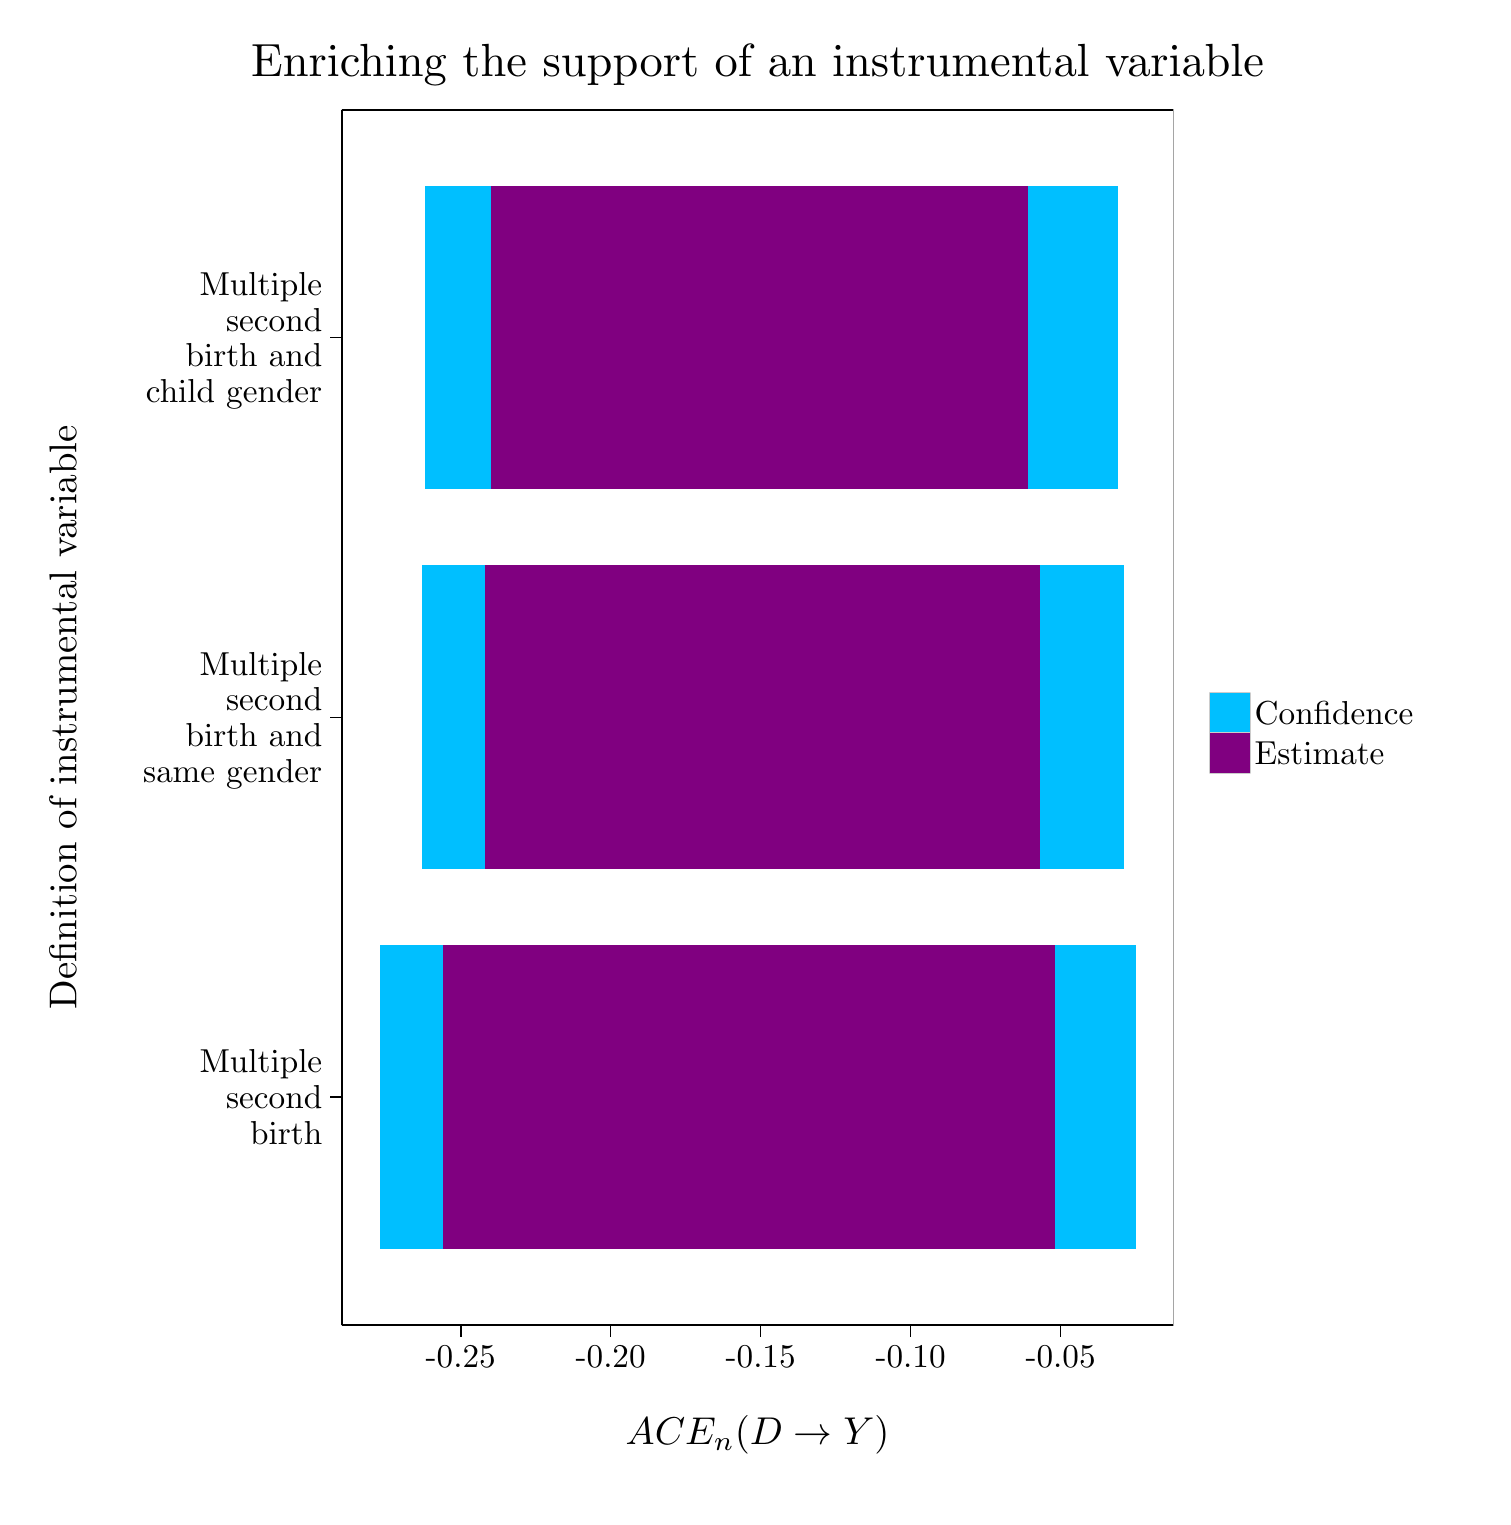
\begin{tikzpicture}[x=1pt,y=1pt]
\definecolor[named]{fillColor}{rgb}{1.00,1.00,1.00}
\path[use as bounding box,fill=fillColor,fill opacity=0.00] (-20,-25) rectangle (505.89,505.89);
\begin{scope}
\path[clip] ( 93.55, 37.06) rectangle (393.99,476.25);
\definecolor[named]{fillColor}{rgb}{0.00,0.75,1.00}

\path[fill=fillColor] (107.21, 64.51) rectangle (380.34,174.31);

\path[fill=fillColor] (122.38,201.76) rectangle (376.00,311.56);

\path[fill=fillColor] (123.47,339.01) rectangle (373.83,448.80);
\definecolor[named]{fillColor}{rgb}{0.50,0.00,0.50}

\path[fill=fillColor] (129.97, 64.51) rectangle (351.07,174.31);

\path[fill=fillColor] (145.14,201.76) rectangle (345.65,311.56);

\path[fill=fillColor] (147.31,339.01) rectangle (341.32,448.80);
\definecolor[named]{drawColor}{rgb}{0.00,0.00,0.00}

\path[draw=drawColor,line width= 0.6pt,line join=round,line cap=round] ( 93.55, 37.06) rectangle (393.99,476.25);
\end{scope}
\begin{scope}
\path[clip] (-20,-25) rectangle (505.89,505.89);
\definecolor[named]{drawColor}{rgb}{0.00,0.00,0.00}

\path[draw=drawColor,line width= 0.6pt,line join=round] ( 93.55, 37.06) --
	( 93.55,476.25);
\end{scope}
\begin{scope}
\path[clip] (-20,-25) rectangle (505.89,505.89);
\definecolor[named]{drawColor}{rgb}{0.00,0.00,0.00}

\node[text=drawColor,anchor=base east,inner sep=0pt, outer sep=0pt, scale=  1.20] at ( 86.44,128.24) {Multiple };

\node[text=drawColor,anchor=base east,inner sep=0pt, outer sep=0pt, scale=  1.20] at ( 86.44,115.28) { second };

\node[text=drawColor,anchor=base east,inner sep=0pt, outer sep=0pt, scale=  1.20] at ( 86.44,102.32) { birth};

\node[text=drawColor,anchor=base east,inner sep=0pt, outer sep=0pt, scale=  1.20] at ( 86.44,271.97) {Multiple };

\node[text=drawColor,anchor=base east,inner sep=0pt, outer sep=0pt, scale=  1.20] at ( 86.44,259.01) { second };

\node[text=drawColor,anchor=base east,inner sep=0pt, outer sep=0pt, scale=  1.20] at ( 86.44,246.05) { birth and };

\node[text=drawColor,anchor=base east,inner sep=0pt, outer sep=0pt, scale=  1.20] at ( 86.44,233.09) { same gender};

\node[text=drawColor,anchor=base east,inner sep=0pt, outer sep=0pt, scale=  1.20] at ( 86.44,409.21) {Multiple };

\node[text=drawColor,anchor=base east,inner sep=0pt, outer sep=0pt, scale=  1.20] at ( 86.44,396.25) { second };

\node[text=drawColor,anchor=base east,inner sep=0pt, outer sep=0pt, scale=  1.20] at ( 86.44,383.29) { birth and };

\node[text=drawColor,anchor=base east,inner sep=0pt, outer sep=0pt, scale=  1.20] at ( 86.44,370.33) { child gender};
\end{scope}
\begin{scope}
\path[clip] (-20,-25) rectangle (505.89,505.89);
\definecolor[named]{drawColor}{rgb}{0.00,0.00,0.00}

\path[draw=drawColor,line width= 0.6pt,line join=round] ( 89.28,119.41) --
	( 93.55,119.41);

\path[draw=drawColor,line width= 0.6pt,line join=round] ( 89.28,256.66) --
	( 93.55,256.66);

\path[draw=drawColor,line width= 0.6pt,line join=round] ( 89.28,393.90) --
	( 93.55,393.90);
\end{scope}
\begin{scope}
\path[clip] (-20,-25) rectangle (505.89,505.89);
\definecolor[named]{drawColor}{rgb}{0.00,0.00,0.00}

\path[draw=drawColor,line width= 0.6pt,line join=round] ( 93.55, 37.06) --
	(393.99, 37.06);
\end{scope}
\begin{scope}
\path[clip] (-20,-25) rectangle (505.89,505.89);
\definecolor[named]{drawColor}{rgb}{0.00,0.00,0.00}

\path[draw=drawColor,line width= 0.6pt,line join=round] (136.47, 32.80) --
	(136.47, 37.06);

\path[draw=drawColor,line width= 0.6pt,line join=round] (190.66, 32.80) --
	(190.66, 37.06);

\path[draw=drawColor,line width= 0.6pt,line join=round] (244.86, 32.80) --
	(244.86, 37.06);

\path[draw=drawColor,line width= 0.6pt,line join=round] (299.05, 32.80) --
	(299.05, 37.06);

\path[draw=drawColor,line width= 0.6pt,line join=round] (353.24, 32.80) --
	(353.24, 37.06);
\end{scope}
\begin{scope}
\path[clip] (-20,-25) rectangle (505.89,505.89);
\definecolor[named]{drawColor}{rgb}{0.00,0.00,0.00}

\node[text=drawColor,anchor=base,inner sep=0pt, outer sep=0pt, scale=  1.20] at (136.47, 21.69) {-0.25};

\node[text=drawColor,anchor=base,inner sep=0pt, outer sep=0pt, scale=  1.20] at (190.66, 21.69) {-0.20};

\node[text=drawColor,anchor=base,inner sep=0pt, outer sep=0pt, scale=  1.20] at (244.86, 21.69) {-0.15};

\node[text=drawColor,anchor=base,inner sep=0pt, outer sep=0pt, scale=  1.20] at (299.05, 21.69) {-0.10};

\node[text=drawColor,anchor=base,inner sep=0pt, outer sep=0pt, scale=  1.20] at (353.24, 21.69) {-0.05};
\end{scope}
\begin{scope}
\path[clip] (-20,-25) rectangle (505.89,505.89);
\definecolor[named]{drawColor}{rgb}{0.00,0.00,0.00}

\node[text=drawColor,anchor=base,inner sep=0pt, outer sep=0pt, scale=  1.40] at (243.77, -6.02) {$ACE_n(D\rightarrow Y)$};
\end{scope}
\begin{scope}
\path[clip] (-20,-25) rectangle (505.89,505.89);
\definecolor[named]{drawColor}{rgb}{0.00,0.00,0.00}

\node[text=drawColor,rotate= 90.00,anchor=base,inner sep=0pt, outer sep=0pt, scale=  1.40] at ( -2.40,256.66) {Definition of instrumental variable};
\end{scope}
\begin{scope}
\path[clip] (-20,-25) rectangle (505.89,505.89);
\definecolor[named]{fillColor}{rgb}{1.00,1.00,1.00}

\path[fill=fillColor] (402.86,232.27) rectangle (484.98,281.05);
\end{scope}
\begin{scope}
\path[clip] (-20,-25) rectangle (505.89,505.89);
\definecolor[named]{drawColor}{rgb}{0.80,0.80,0.80}
\definecolor[named]{fillColor}{rgb}{1.00,1.00,1.00}

\path[draw=drawColor,line width= 0.6pt,line join=round,line cap=round,fill=fillColor] (407.13,250.99) rectangle (421.58,265.44);
\end{scope}
\begin{scope}
\path[clip] (-20,-25) rectangle (505.89,505.89);
\definecolor[named]{fillColor}{rgb}{0.00,0.75,1.00}

\path[fill=fillColor] (407.13,250.99) rectangle (421.58,265.44);

\path[] (407.13,250.99) --
	(421.58,265.44);
\end{scope}
\begin{scope}
\path[clip] (-20,-25) rectangle (505.89,505.89);
\definecolor[named]{fillColor}{rgb}{0.00,0.75,1.00}

\path[fill=fillColor] (407.13,250.99) rectangle (421.58,265.44);

\path[] (407.13,250.99) --
	(421.58,265.44);
\end{scope}
\begin{scope}
\path[clip] (-20,-25) rectangle (505.89,505.89);
\definecolor[named]{drawColor}{rgb}{0.80,0.80,0.80}
\definecolor[named]{fillColor}{rgb}{1.00,1.00,1.00}

\path[draw=drawColor,line width= 0.6pt,line join=round,line cap=round,fill=fillColor] (407.13,236.53) rectangle (421.58,250.99);
\end{scope}
\begin{scope}
\path[clip] (-20,-25) rectangle (505.89,505.89);
\definecolor[named]{fillColor}{rgb}{0.50,0.00,0.50}

\path[fill=fillColor] (407.13,236.53) rectangle (421.58,250.99);

\path[] (407.13,236.53) --
	(421.58,250.99);
\end{scope}
\begin{scope}
\path[clip] (-20,-25) rectangle (505.89,505.89);
\definecolor[named]{fillColor}{rgb}{0.50,0.00,0.50}

\path[fill=fillColor] (407.13,236.53) rectangle (421.58,250.99);

\path[] (407.13,236.53) --
	(421.58,250.99);
\end{scope}
\begin{scope}
\path[clip] (-20,-25) rectangle (505.89,505.89);
\definecolor[named]{drawColor}{rgb}{0.00,0.00,0.00}

\node[text=drawColor,anchor=base west,inner sep=0pt, outer sep=0pt, scale=  1.20] at (423.39,254.08) {Confidence};
\end{scope}
\begin{scope}
\path[clip] (-20,-25) rectangle (505.89,505.89);
\definecolor[named]{drawColor}{rgb}{0.00,0.00,0.00}

\node[text=drawColor,anchor=base west,inner sep=0pt, outer sep=0pt, scale=  1.20] at (423.39,239.63) {Estimate};
\end{scope}
\begin{scope}
\path[clip] (-20,-25) rectangle (505.89,505.89);
\definecolor[named]{drawColor}{rgb}{0.00,0.00,0.00}

\node[text=drawColor,anchor=base,inner sep=0pt, outer sep=0pt, scale=  1.68] at (243.77,488.30) {Enriching the support of an instrumental variable};
\end{scope}
\end{tikzpicture}
